\documentclass[a0paper, twocolumn, csc, english, final]{mpi2015_poster}

\definecolor{clustercassis} {cmyk}{0.30, 1.00, 0.00, 0.05}
\definecolor{clusterblue} {cmyk}{1.00, 0.00, 0.10, 0.00}
\colorlet{CEmphasis1}{clustercassis}
\colorlet{CEmphasis2}{clusterblue}

\usepackage{lipsum}
\usepackage{blindtext}
\usepackage{tcolorbox}
\usepackage{amsmath}
\usepackage{derivative}
\usepackage{hyperref}
\hypersetup{
	colorlinks,
	citecolor=black,
	urlcolor=MPIblue,
}
\usepackage{minted}
\usepackage{newtxsf}

\usepackage[table]{xcolor}
\usepackage{tikz}
\usetikzlibrary{arrows.meta, calc, positioning, shapes.geometric}

\usepackage[font=small,labelfont=bf]{caption}

\title{Improving Interoperability in Scientific Computing\\via MaRDI Open Interfaces}
\author{Dmitry I.\ Kabanov}
\author{Stephan Rave}
\author{Mario Ohlberger}
\affil{Institute for Analysis and Numerics, University of Münster, Münster, Germany}

\newcommand{\OIF}{\textsc{MaRDI Open Interfaces}\xspace}

\graphicspath{{./assets/}}

\usepackage[natbib=true, style=authoryear, giveninits=true, uniquename=init]{biblatex}
% While editing, it is convenient to use an external BIB file,
% which is, nevertheless, is not commited to the Git repository.
% To extract only used citations and put them to `bibliography`,
% use this command in the terminal:
% jabref --nogui --aux main.aux,bibliography.bib bibliography-external.bib
\IfFileExists{./bibliography-external.bib}{%
	\addbibresource{bibliography-external.bib}
}{%
	\addbibresource{bibliography.bib}
}

\partnerlogos{
  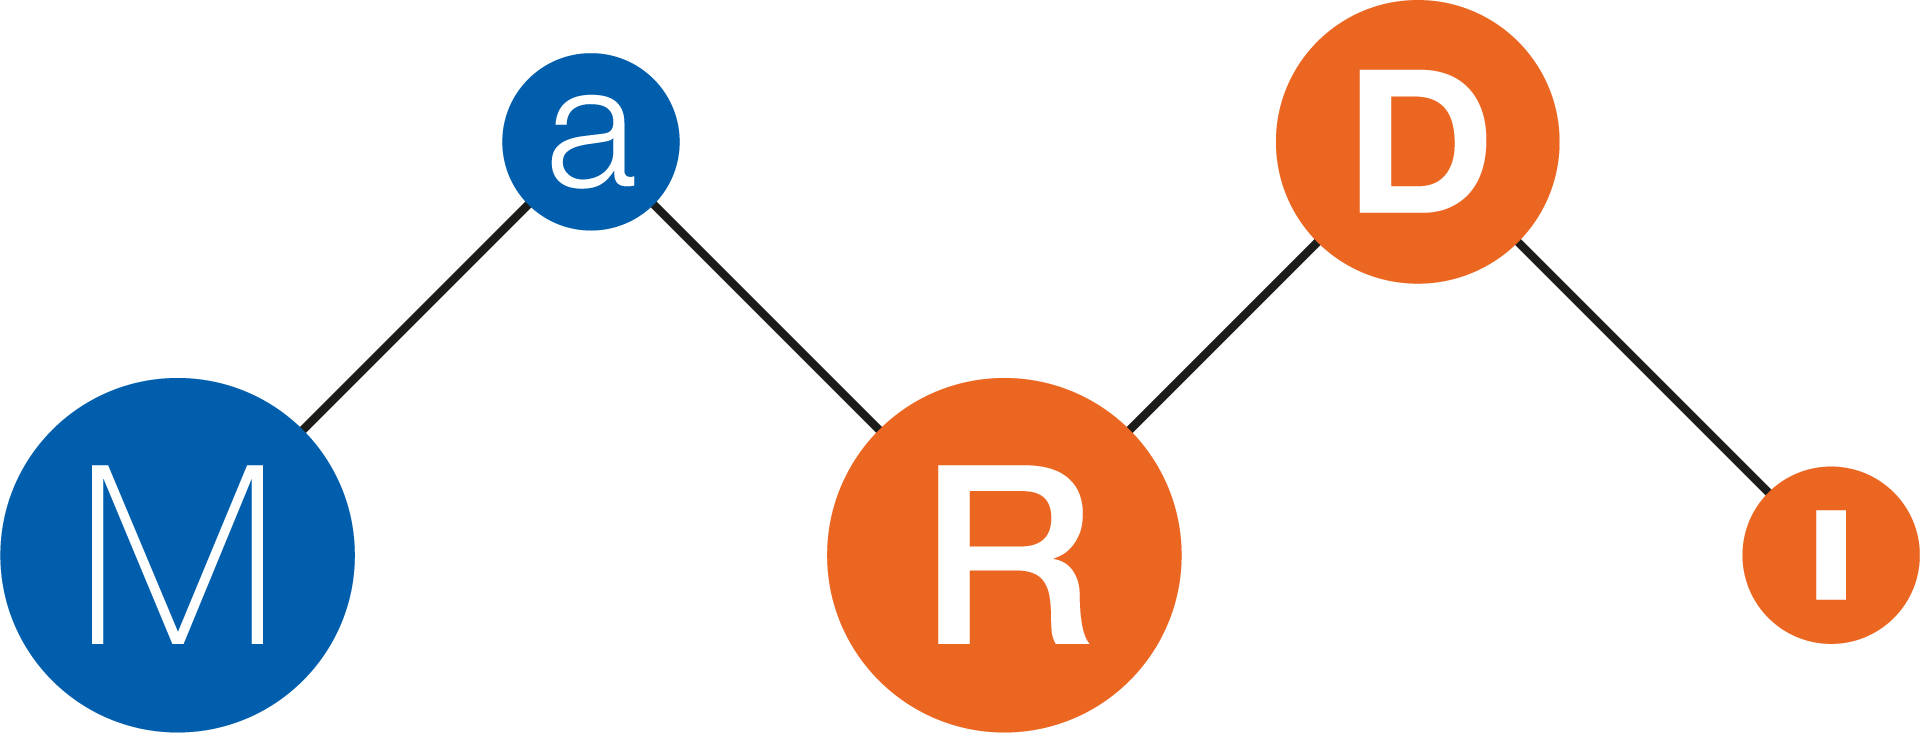
\includegraphics[height=\logoheight]{logos/MaRDI_Logo_L_5_rgba_cropped.png} \hspace{3ex}
  
\includegraphics[height=\logoheight]{logos/poster_wwumlogo_cropped.pdf}
}


\begin{document}
\begin{poster}
  \begin{pcolumn}
    \makesection{Summary}
    \begin{pbox}
      \large
      Computational scientists often face two obstacles while conducting
      numerical experiments:
      \begin{itemize}
        \item Multiple programming languages are used for numerical solvers
        \item Multiple solvers have different interfaces
              for the same problem types
      \end{itemize}

      Combination of solvers, thus, could lead to significant programming effort
      on scientist's side: \textbf{writing bindings}
      and \textbf{adapting interfaces}.
      \OIF{} aim to improve interoperability in Scientific
      Computing by alleviating these obstacles by replacing pairwise bindings
      between languages and implementations with decoupled bindings.

      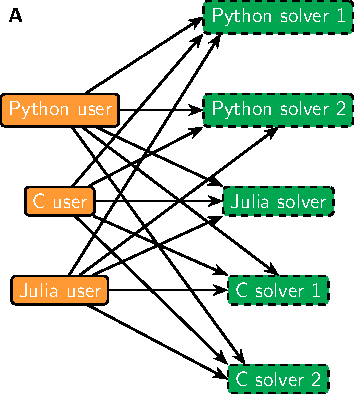
\includegraphics[width=0.46\columnwidth]{tikz/pairwise_bindings}
      \hfill
      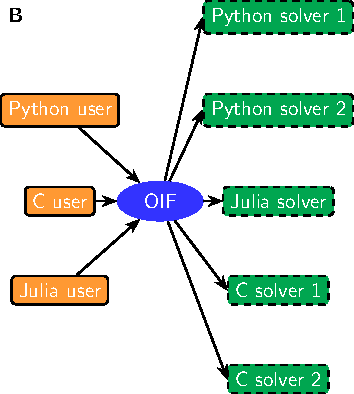
\includegraphics[width=0.46\columnwidth]{tikz/oif_bindings}
      \captionof{figure}{%
        Schematic comparison of two approaches to the problem
        of multiple languages/multiple implementations.
        \textbf{A}~Standard pairwise bindings\quad
        \textbf{B}~Bindings via MaRDI Open Interfaces.
      }

      % Our \textbf{objectives} during the project are:
      % \begin{itemize}
      % \end{itemize}

  % Objectives
      \begin{center}
        \begin{tcolorbox}[
          colback=white, colframe=mardiblue, parbox=true,
          left=1em, right=1em,
                    before={\par\bigskip\noindent}, after={\par\bigskip},  width=\columnwidth]
  {\Large\color{mardiblue}Objectives\medskip}
  \begin{itemize}
        \item Develop library that passes data between languages automatically
        \item Develop generic interfaces for typical numerical problems
        \item Encourage the community to program against these interfaces
  \end{itemize}
  \end{tcolorbox}
  \end{center}

      Similar to software packages such as \textsc{PyMOR}~\citep{Milk2016},
      \textsc{SUNDIALS}~\citep{GardnerEtAl2022},
      or \textsc{PreCICE}~\citep{Chourdakis2022},
      we aim to abstract out discrepancies between
      different solvers, so that computational scientists would spend less time
      connecting them.

    \end{pbox}

    \makesection{Software Architecture and Data Flow}
    \begin{pbox}
      \large
      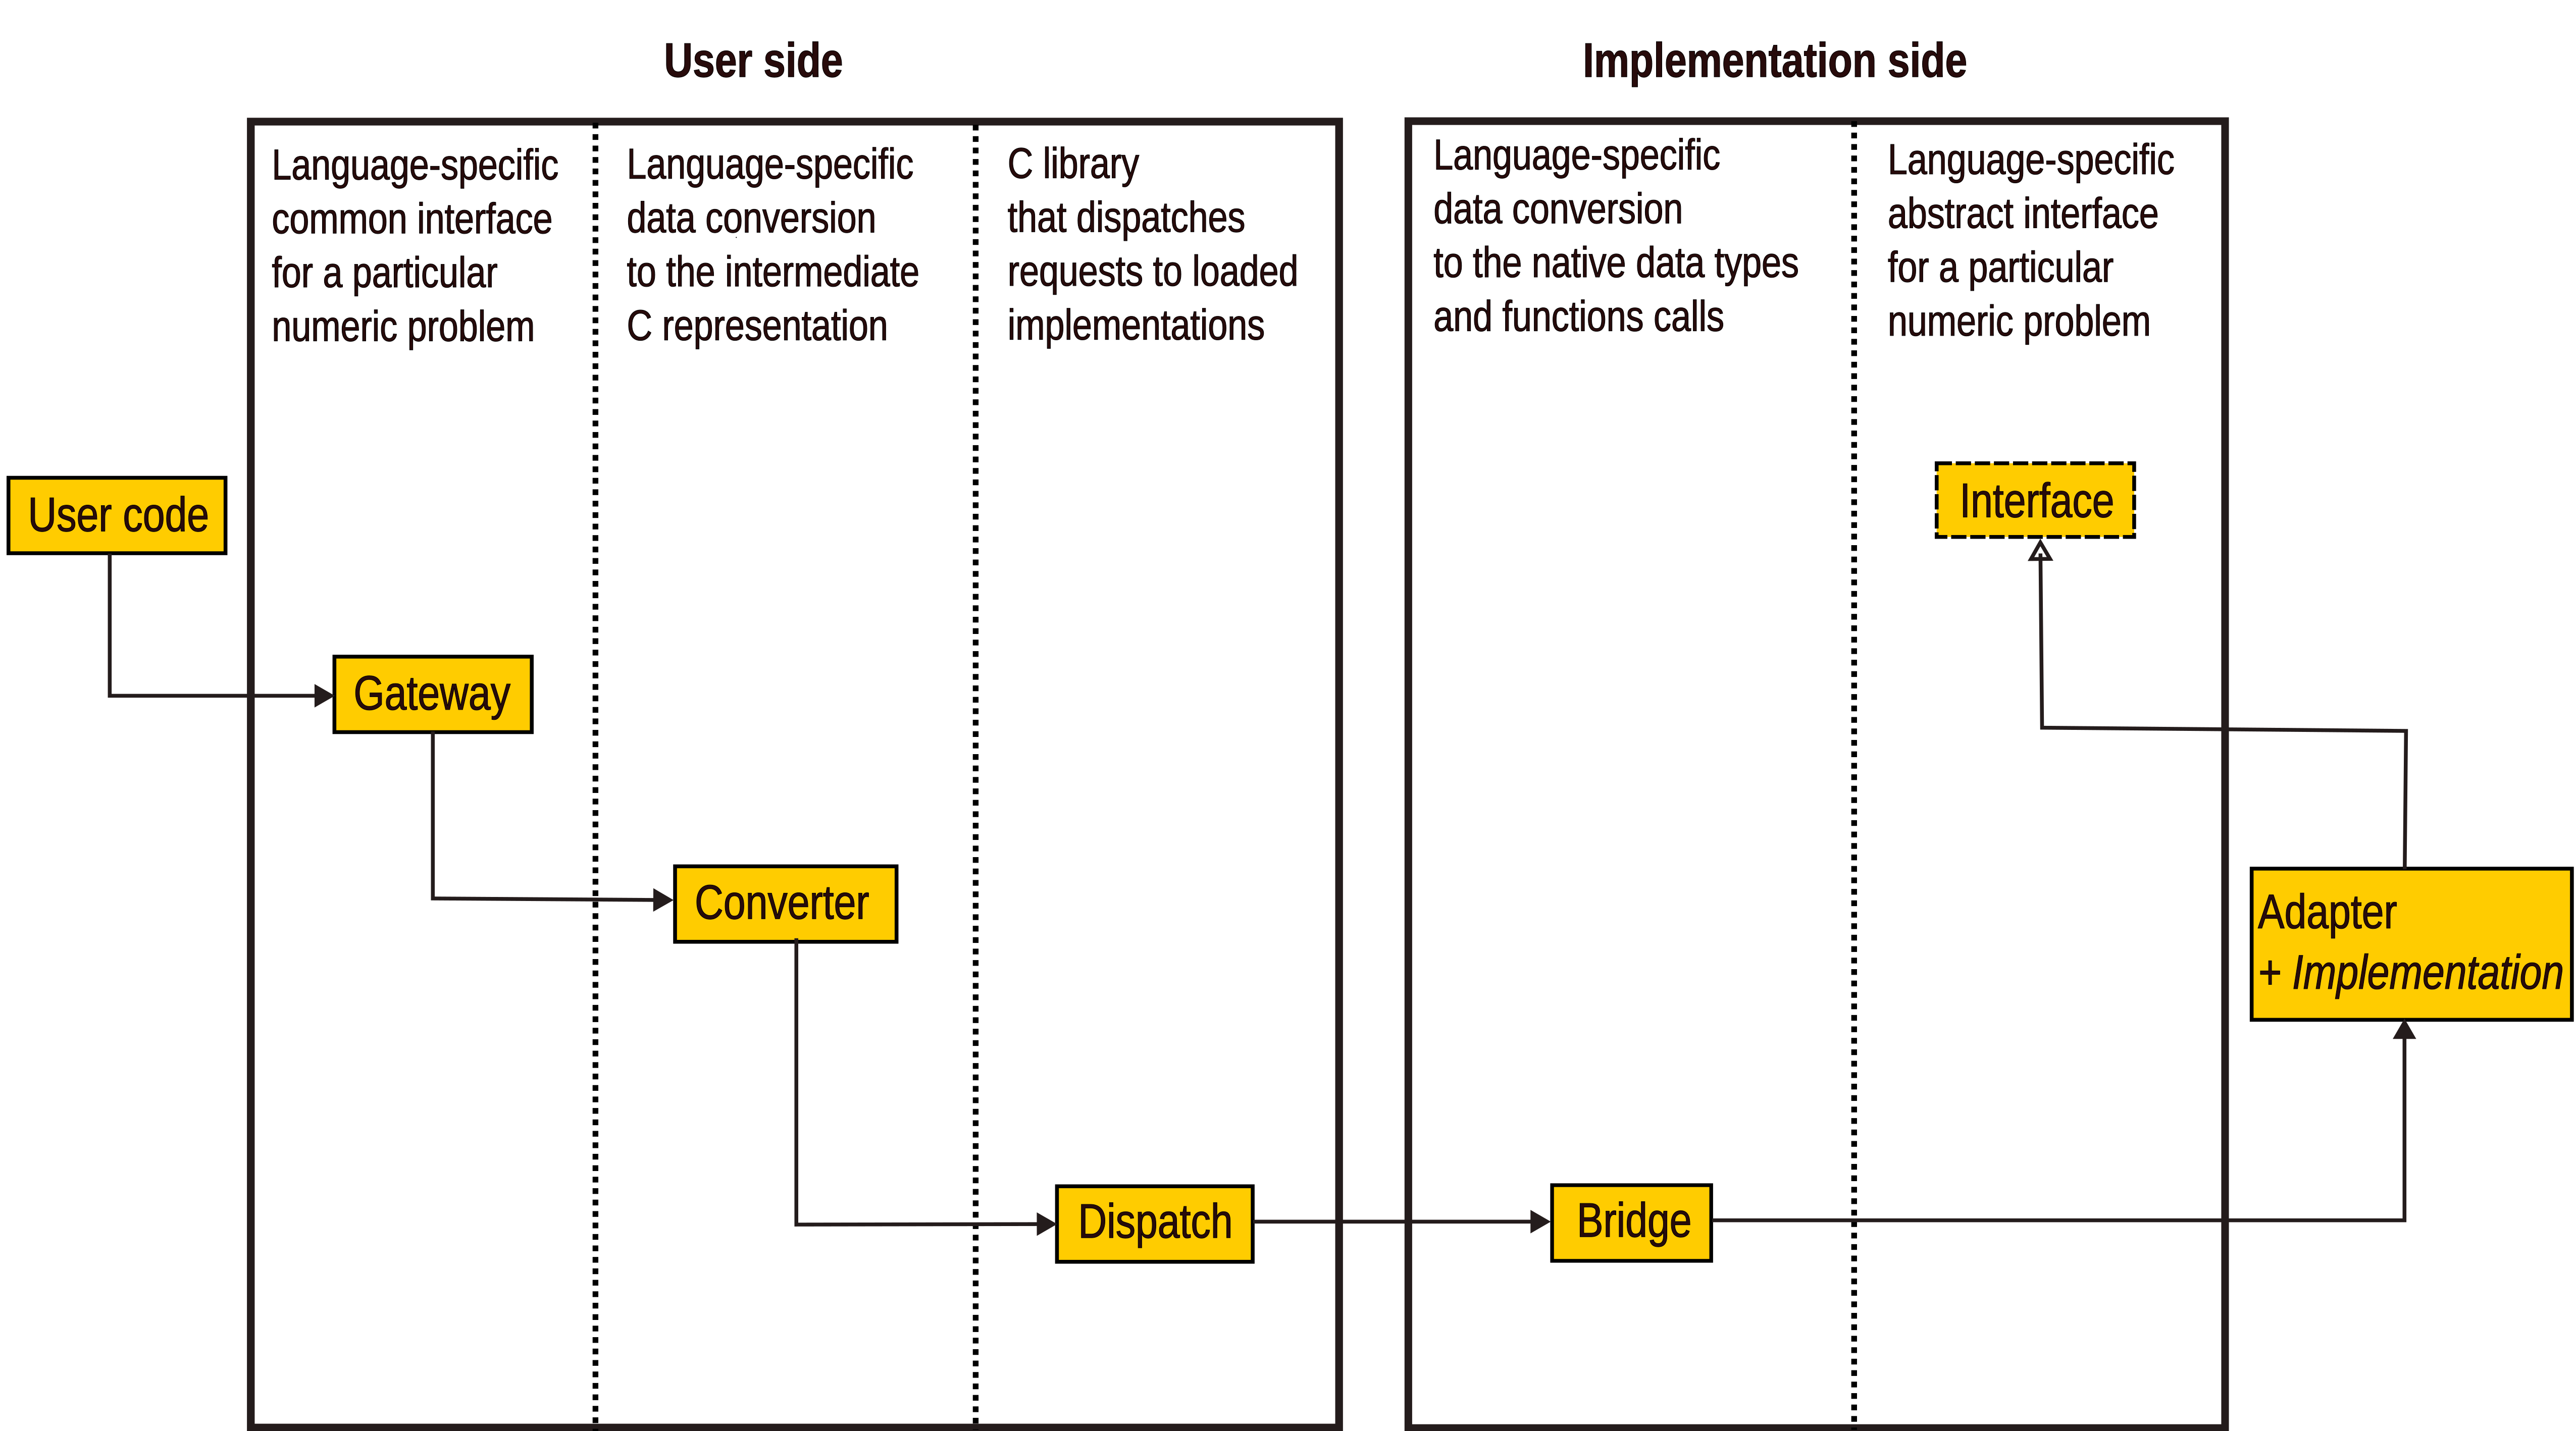
\includegraphics[width=\columnwidth]{arch}

      % \textbf{User} requests an implementation of an Open Interface
      % and interacts with the implementation only via a \textbf{Gateway},
      % so that the discrepancies between different implementations in terms
      % of functions signatures and order of invocation become transparent
      % to the \textbf{User}.

      % The function arguments are converted from the user's language
      % to a C intermediate representation inside a \textbf{Converter}
      % that passes them further.
      % The \textbf{Dispatch} is responsible for loading an implementation
      % and its corresponding runtime (\textbf{Bridge}).
      % The \textbf{Bridge} converts data from the intermediate representation
      % to the native data types of the implementation and invokes
      % the requested function, which also occurs via \textbf{Interface},
      % that is, the implementation is invoked via an adapter.
    \end{pbox}

    \makesection{Acknowledgments}
    \begin{pbox}
      \large
      The authors would like to thank for the provided funding
      the National Research Data Infrastructure,
      project number~460135501, NFDI~29/1 “MaRDI – Mathematical
      Research Data Initiative”
      and
      the German Research Foundation,
      Germany's Excellence Strategy EXC~2044-390685587,
      ``Mathematics Münster: Dynamics--Geometry--Structure''.
    \end{pbox}
  \end{pcolumn}
  % Right column.
  \begin{pcolumn}
    \makesection{Example usage}
    \begin{pbox}
      \large
      Consider the inviscid Burgers' equation problem:
      \begin{align*}
         & \pdv{u}{t} + \pdv{\left( u^{2} / 2 \right)}{x} = 0,
        \quad t \in [0, 2], \quad x \in [0, 2]                 \\
         & u(t, 0) = 0.5 - 0.25 \sin \left( \pi x \right) \mbox{ and }
         u(t, 0) = u(t, 2),
      \end{align*}
      \begin{minipage}{\dimexpr0.58\columnwidth - 2\tabcolsep}
        which we integrate in time
        using an open interface
        for Initial-Value Problems (\texttt{IVP}) for ordinary
        differential equations.

        \vspace{0.5em}
        \captionof{figure}{%
          Solution of the Burgers' problem using open interface \texttt{IVP}
          with three implementations:
          \textsc{Sundials CVODE},
          \textsc{SciPy},
          and~\textsc{OrdinaryDiffEq.jl}
        }
      \end{minipage}\hfill%
      \begin{minipage}{\dimexpr0.42\columnwidth - 2\tabcolsep}
        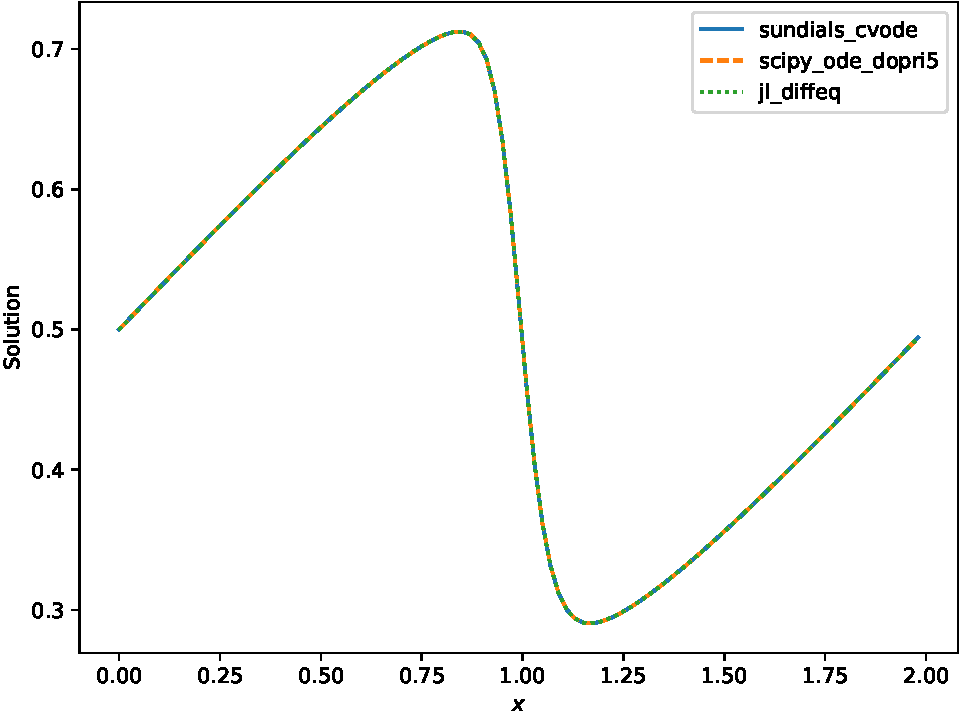
\includegraphics{ivp_c_burgers_eq}
      \end{minipage}

      \vspace{0.5em}
      \textbf{User code in Python:}
      \begin{minted}[autogobble, beameroverlays, escapeinside=||]{Python}
        from oif.interfaces.ivp import IVP
        ...

        # `BurgersEquationProblem` is a utility user class.
        impl = "scipy_ode"  # or "sundials_cvode", or "jl_diffeq"
        problem = BurgersEquationProblem(N=1001)
        s = IVP(impl)
        s.set_initial_value(problem.y0, problem.t0)
        s.set_rhs_fn(problem.compute_rhs)

        times = np.linspace(problem.t0, problem.tfinal, num=11)

        soln = [y0]
        for t in times[1:]:
            s.integrate(t)
            soln.append(s.y)
      \end{minted}
    \end{pbox}
    \makesection{Performance study}
    \begin{pbox}

      \begin{minipage}{\dimexpr0.58\columnwidth - 2\tabcolsep}
        \centering
      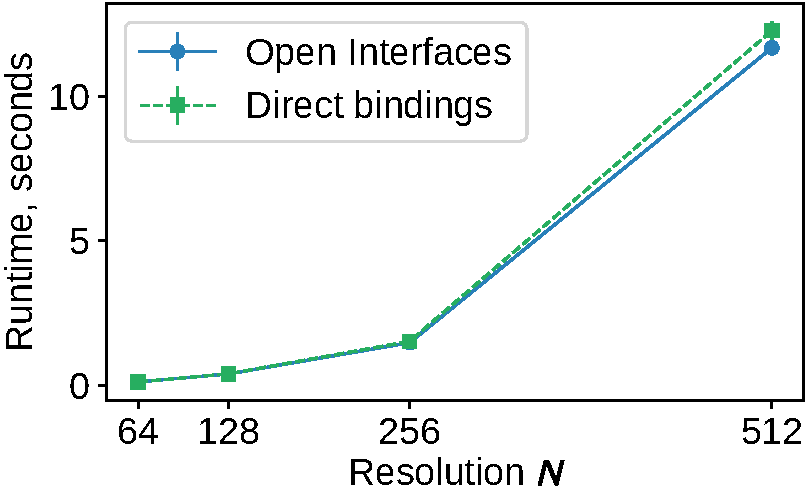
\includegraphics[width=0.8\columnwidth]{ivp_cvode_gs_performance}
      \end{minipage}\hfill%
      \begin{minipage}{\dimexpr0.42\columnwidth - 2\tabcolsep}
        Do \OIF{} sacrifice high-performance computing? We integrate
        a 2D Gray--Scott reaction--diffusion system using \OIF{}
        and~\textsc{Sundials CVODE} solver and using the same solver
        via direct bindings (from Python).

        \captionof{figure}{Comparison of runtimes between using the same solver
          via \textsc{Open Interfaces} and directly.
          Error bars are standard deviations of 30 runs.}
      \end{minipage}
    \end{pbox}
    \makesection{Conclusions}
    \begin{pbox}
      \large
      We demonstrated how \OIF{} can be used to improve
      interoperability in Scientific Computing.
      Using this software package, computational scientists can connect numerical
      solvers written in different languages, without explicitly writing bindings
      to these solvers, enabling complex experiment workflows.

      Besides, the library allows switching between different implementations
      of a numerical algorithm without extensive modifications of user's code,
      which facilitates benchmarking numerical software in terms of performance
      and correctness.
    \end{pbox}
    \makesection{Selected References}
    \begin{pbox}
      \vspace{1em}
      \defbibheading{bibliography}{} % Remove default "References" heading.
      \printbibliography[]
      % Chourdakis, G. et al. (2022). “preCICE v2: A sustainable and user-friendly coupling library”. In:
      % \emph{Open Research Europe} 2, p. 51. DOI: 10.12688/openreseurope.14445.2.
      % \vspace{0.5em}
      % Gardner, D. J. et al. (2022). “Enabling New Flexibility in the SUNDIALS Suite of Nonlinear and
      % Differential/Algebraic Equation Solvers”. In: \emph{ACM Transactions on Mathematical Software} 48.3,
      % pp. 1–24. DOI: 10.1145/3539801.
      % \vspace{0.5em}
      % Milk, R., S. Rave, and F. Schindler (2016). “pyMOR – Generic Algorithms and Interfaces for Model
      % Order Reduction”. In: \emph{SIAM Journal on Scientific Computing} 38.5, S194–S216.
      % DOI: 10.1137/15m1026614.
    \end{pbox}
  \end{pcolumn}
\end{poster}
\end{document}
